\documentclass{jsarticle}

\usepackage{graphicx}
\usepackage{amsmath,amssymb,bm}
\usepackage{algorithm,algpseudocode}
\include{preamble}

\everymath{\displaystyle}

\title{\bf DIRECT法}
\author{\Large{\bf 杉原 知道}}

\begin{document}
\maketitle

\section{はじめに}

次の最小化問題を考えます.
\begin{align*}
f(\bm{x})\rightarrow\mbox{min.}\quad\mbox{subject to}\quad \bm{x}\in\left\{
\bm{x}\left|
x_{\mathrm{min}j}\leq x_{j}\leq x_{\mathrm{max}j}\quad\mbox{for}~\forall j=1,\cdots,n
\right.\right\}
\end{align*}
ただし,
$f$は目的関数,
$\bm{x}=[x_{1}~\cdots~x_{n}]^{\mathrm{T}}$は設計変数,
$x_{\mathrm{min}j}$および$x_{\mathrm{max}j}$は$x_{j}$の下限値および上限値です.
$f$はこの探索空間においてLipschitz連続である(つまり勾配が無限大となる尖った点を持たない)ものと仮定します.

$x_{j}$($j=1,\cdots,n$)を$x_{\mathrm{max}j}-x_{\mathrm{min}j}$で正規化し,
適当な変数変換を用いて$f$を置き換えれば,
探索空間は単位超正方形となります.
すなわち$x_{\mathrm{min}j}=0$,$x_{\mathrm{max}j}=1$としても一般性を失いません.
以降はこれを前提とします.

DIRECT法(DIviding RECTangle method)は,
\begin{enumerate}
\item{探索空間の超長方形群への分割}
\item{超長方形領域群からの探索空間の選択(潜在的最適領域の抽出)}
\end{enumerate}
の二つのプロセスを反復することで最小点が存在する領域を絞り込んでいく,
ブラックボックス最適化の一種で,次の文献が出典です.
\begin{quote}
D. R. Jones, C. D. Perttunen and B. E. Stuckman,
Lipschizian Optimization Without the Lipschitz Constant,
Journal of Optimization Theory and Application, Vol. 79, No. 1, pp. 157--181, 1993.
\end{quote}
考え方も実装も比較的分かりやすいのですが,
日本語の解説が見当たらないので書いてみました.
次の文献も参考にしました.
\begin{quote}
J. Gablonsky, An Implementation of the {\tt DIRECT} algorithm, Technial report of North Carolina State University, 1998.
\end{quote}



\section{探索空間の超長方形群への分割}

探索空間の分割は再帰的に行われます.
既にある程度反復計算が進み,
探索空間(単位超正方形)が幾つかの超長方形領域に分割されている状況から考え始めましょう.
$i$番目領域の中心座標を$\bm{x}_{\mathrm{C}i}$,
各辺の長さを$\{d_{ij}\}$($j=1,\cdots,n$)とおき,
$d_{i}=\max_{j}\{d_{ij}\}$とします.
分割は$d_{ij}=d_{i}$,つまり長さ最大である辺の方向に行います.
そのような辺のインデックスの集合を$\mathcal{I}_{i}$とおきましょう.
例えば下図に示した場合は$d_{i}=d_{i1}=d_{i2}>d_{i3}$なので,$\mathcal{I}_{i}=\{1,2\}$です.

\begin{figure}[h]
\begin{center}
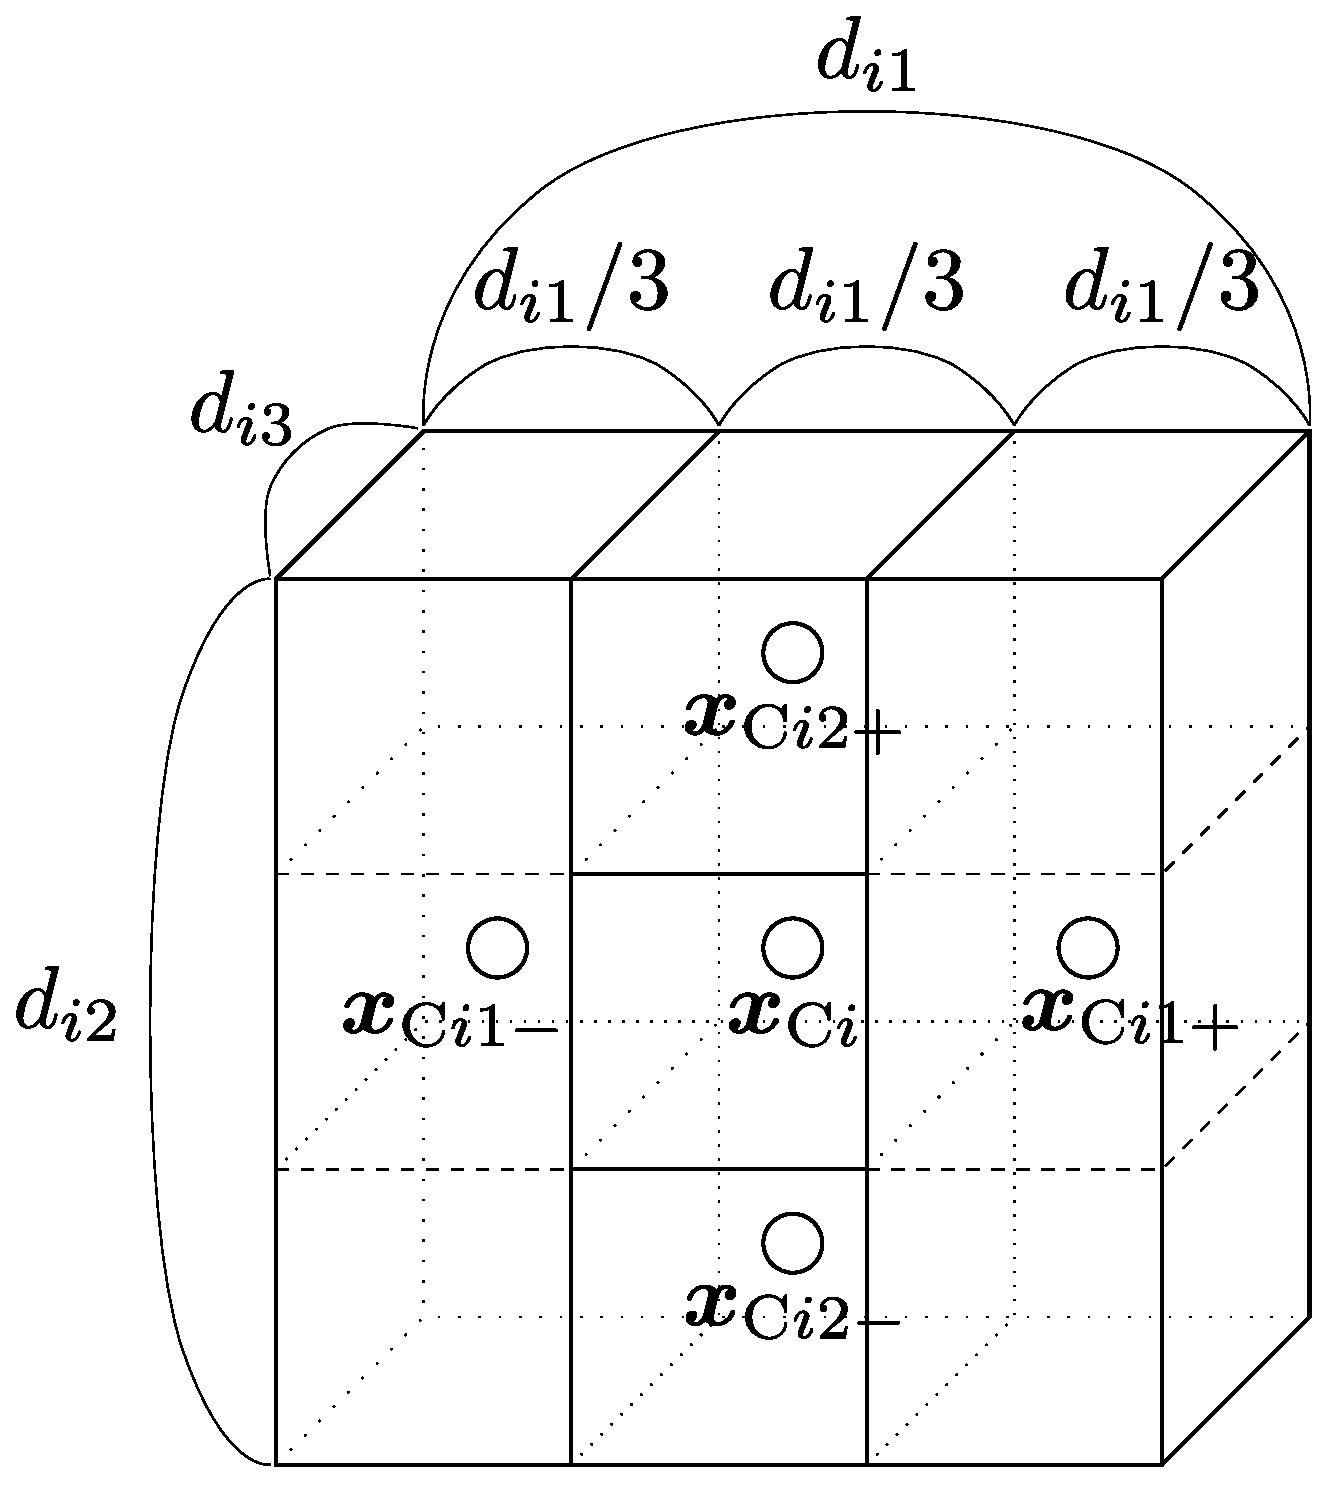
\includegraphics[width=.4\textwidth]{fig/DIRECT_divide.eps}
\end{center}
\end{figure}

$\mathcal{I}_{i}$の全ての成分$j$について,
$\bm{x}_{\mathrm{C}ij+}=\bm{x}_{\mathrm{C}i}+(d_{i}/3)\bm{e}_{j}$および
$\bm{x}_{\mathrm{C}ij-}=\bm{x}_{\mathrm{C}i}-(d_{i}/3)\bm{e}_{j}$における目的関数の値
$f_{ij+}=f(\bm{x}_{\mathrm{C}ij+})$および$f_{ij-}=f(\bm{x}_{\mathrm{C}ij-})$を求めます.
ただし,$\bm{e}_{j}$は$j$番目成分のみが1,他は全て0の$n$次元ベクトルです.
$w_{ij}=\min\{f_{ij+},f_{ij-}\}$とし,
領域をまず最小の$w_{ij}$を与える$j$の方向に3等分割します.
次にそれらの中央の領域を,
2番目に小さい$w_{ij}$を与える$j$の方向に3等分割します.
残りの$\mathcal{I}_{i}$の全ての成分$j$についても同様の手続きを行うことで,
$i$番目領域の分割が完了します.
上図は,$w_{i1}<w_{i2}$である場合の分割の様子を示しています.

全探索領域は辺の長さが全て1である超正方形に正規化されているので,
上記のように分割された超長方形領域の辺の長さは,
ある非負整数$l$を用いて$3^{-l}$と表せます.
$l$を辺の{\bf レベル}と呼ぶことにしましょう.
各辺の長さは各辺のレベルで置き換えられます.
上図の例では,
分割前の超長方形領域の各辺レベルは$\{l,l,l+1\}$であり,
それが分割によってまず
$\{l+1,l,l+1\}$に,
次に$\{l+1,l+1,l+1\}$になっているということです.
このように,一つの超長方形領域の辺レベルは$l$か$l+1$のいずれかであり,
$j$番目の辺の分割によって$j$番目の辺レベルが1増えることになります.
辺レベルの最大値を,{\bf 超長方形領域のレベル}と呼びましょう.
レベル$l$の超長方形を分割したとき,
最後の分割で生成された領域群のみレベルが1増え,超正方形となります.

上記の$i$番目領域に付随する
中心座標$\bm{x}_{\mathrm{C}i}$,
そこにおける評価値$f_{i}=f(\bm{x}_{\mathrm{C}i})$,
そして各辺レベル$\{l_{ij}\}$をまとめて$\bm{\xi}_{i}=(\bm{x}_{\mathrm{C}i},f_{i},\{l_{ij}\})$とおきます.
また,領域のレベルを$l_{i}=\max\{l_{ij}\}$とします.
次節で説明する潜在的最適領域の抽出における便利のために,
これらが同一レベルごとにグルーピングされ,
さらに$f_{i}$に基づいて昇順にソートされているように,
全ての超長方形領域群$\mathcal{R}$を作成します.

以上をまとめたアルゴリズムをAlgorithm \ref{alg:direct_divide}に示します.
Algorithm \ref{alg:direct_insert_index}は,
$\mathcal{I}$を作成するための補助アルゴリズムです.
ただし,$w_{j}$をキーとする挿入ソートを行うために,$\mathcal{I}$は$(j,w_{j})$を要素に持つものとします.
また\textsc{DIRECT\_AddRect}$(\mathcal{R},l,\bm{\xi})$は,
超長方形領域$\bm{\xi}$を$\mathcal{R}$のレベル$l$のグループに$f_{i}$が昇順になるよう追加する関数です
(アルゴリズムは省略します).

\begin{algorithm}[tbh]
\caption{\textsc{DIRECT\_Divide}$(\mathcal{R};l_{i},\bm{\xi}_{i},f)$}
\label{alg:direct_divide}
\begin{algorithmic}[1]
\State $\mathcal{I}\leftarrow\emptyset$
\State $d\leftarrow 3^{-l_{i}}$
\For{$j\leftarrow 1,\cdots,n$}
  \If{$l_{ij}=l_{i}$}
    \State $\bm{x}_{\mathrm{C}ij+}\leftarrow\bm{x}_{\mathrm{C}i}+d\bm{e}_{j}$
    \State $\bm{x}_{\mathrm{C}ij-}\leftarrow\bm{x}_{\mathrm{C}i}-d\bm{e}_{j}$
    \State $f_{ij+}\leftarrow f(\bm{x}_{\mathrm{C}ij+})$
    \State $f_{ij-}\leftarrow f(\bm{x}_{\mathrm{C}ij-})$
    \State \textsc{InsertIndex}$(\mathcal{I};j,\min\{f_{ij+},f_{ij-}\})$
  \EndIf
\EndFor
\For{$(j,w)\in\mathcal{I}$}
  \State $l_{ij}\leftarrow l_{i}+1$
  \State $\bm{\xi}_{ij+}\leftarrow(\bm{x}_{\mathrm{C}ij+},f_{ij+},\{l_{ij}\})$
  \State $\bm{\xi}_{ij-}\leftarrow(\bm{x}_{\mathrm{C}ij-},f_{ij-},\{l_{ij}\})$
  \If{$j=N_{\mathcal{I}}$}
    \State $l_{i}\leftarrow l_{i}+1$
  \EndIf
  \State \textsc{DIRECT\_AddRect}$(\mathcal{R};l_{i},\bm{\xi}_{ij+})$
  \State \textsc{DIRECT\_AddRect}$(\mathcal{R};l_{i},\bm{\xi}_{ij-})$
\EndFor
\State $\bm{\xi}_{i}\leftarrow(\bm{x}_{\mathrm{C}i},f_{i},\{l_{ij}\})$
\State \textsc{DIRECT\_AddRect}$(\mathcal{R};l_{i},\bm{\xi}_{i})$
\end{algorithmic}
\end{algorithm}

\begin{algorithm}[tbh]
\caption{\textsc{InsertIndex}$(\mathcal{I};j,w)$}
\label{alg:direct_insert_index}
\begin{algorithmic}[1]
\For{$k\leftarrow 1,\cdots,N_{\mathcal{I}}$}
  \If{$w>w_{k}$}
    \State break;
  \EndIf
\EndFor
\State \textsc{Insert}$(\mathcal{I};k,(j,w))$
\end{algorithmic}
\end{algorithm}




\section{超長方形領域群からの探索空間の選択(潜在的最適領域の抽出)}

分割によって得られた超長方形領域群から,次に探索する部分超長方形を選ぶ方法を説明します.
前節で述べたように,$\bm{\xi}_{i}\in\mathcal{R}$の各辺の長さは$d_{ij}=3^{-l_{ij}}$になっています.
変数$\tilde{\bm{x}}_{ij}=\tilde{x}_{ij}\bm{e}_{j}$($\tilde{x}_{ij}\in[-d_{ij}/2,d_{ij}/2]$)を定義すると,
$f$が探索空間内部でLipschitz連続であることより,
次を満たす正の係数$\gamma$が存在するはずです.
\begin{align*}
f(\tilde{\bm{x}}_{ij}+\bm{x}_{\mathrm{C}i})&\geq f_{i}-\gamma\tilde{x}_{ij}
& &\mbox{($\tilde{x}_{ij}\geq 0$のとき)}
\\
f(\tilde{\bm{x}}_{ij}+\bm{x}_{\mathrm{C}i})&\geq f_{i}+\gamma\tilde{x}_{ij}
& &\mbox{($\tilde{x}_{ij}< 0$のとき)}
\end{align*}
上2式において$\tilde{x}_{ij}=\pm d_{ij}/2$とすると,次式を得ます.
\begin{align*}
f(d_{ij}\bm{e}_{i}+\bm{x}_{\mathrm{C}i})&\geq f_{i}-\gamma d_{ij}/2
\\
f(-d_{ij}\bm{e}_{i}+\bm{x}_{\mathrm{C}i})&\geq f_{i}-\gamma d_{ij}/2
\end{align*}
したがって,
$i$番目領域内部では
\begin{align*}
f(\bm{x})\geq D_{ij}\overset{\mathrm{def}}{=}f_{i}-\gamma d_{ij}/2
\end{align*}
が言えます.
下の図はこれを説明したものです.

\begin{figure}[h]
\begin{center}
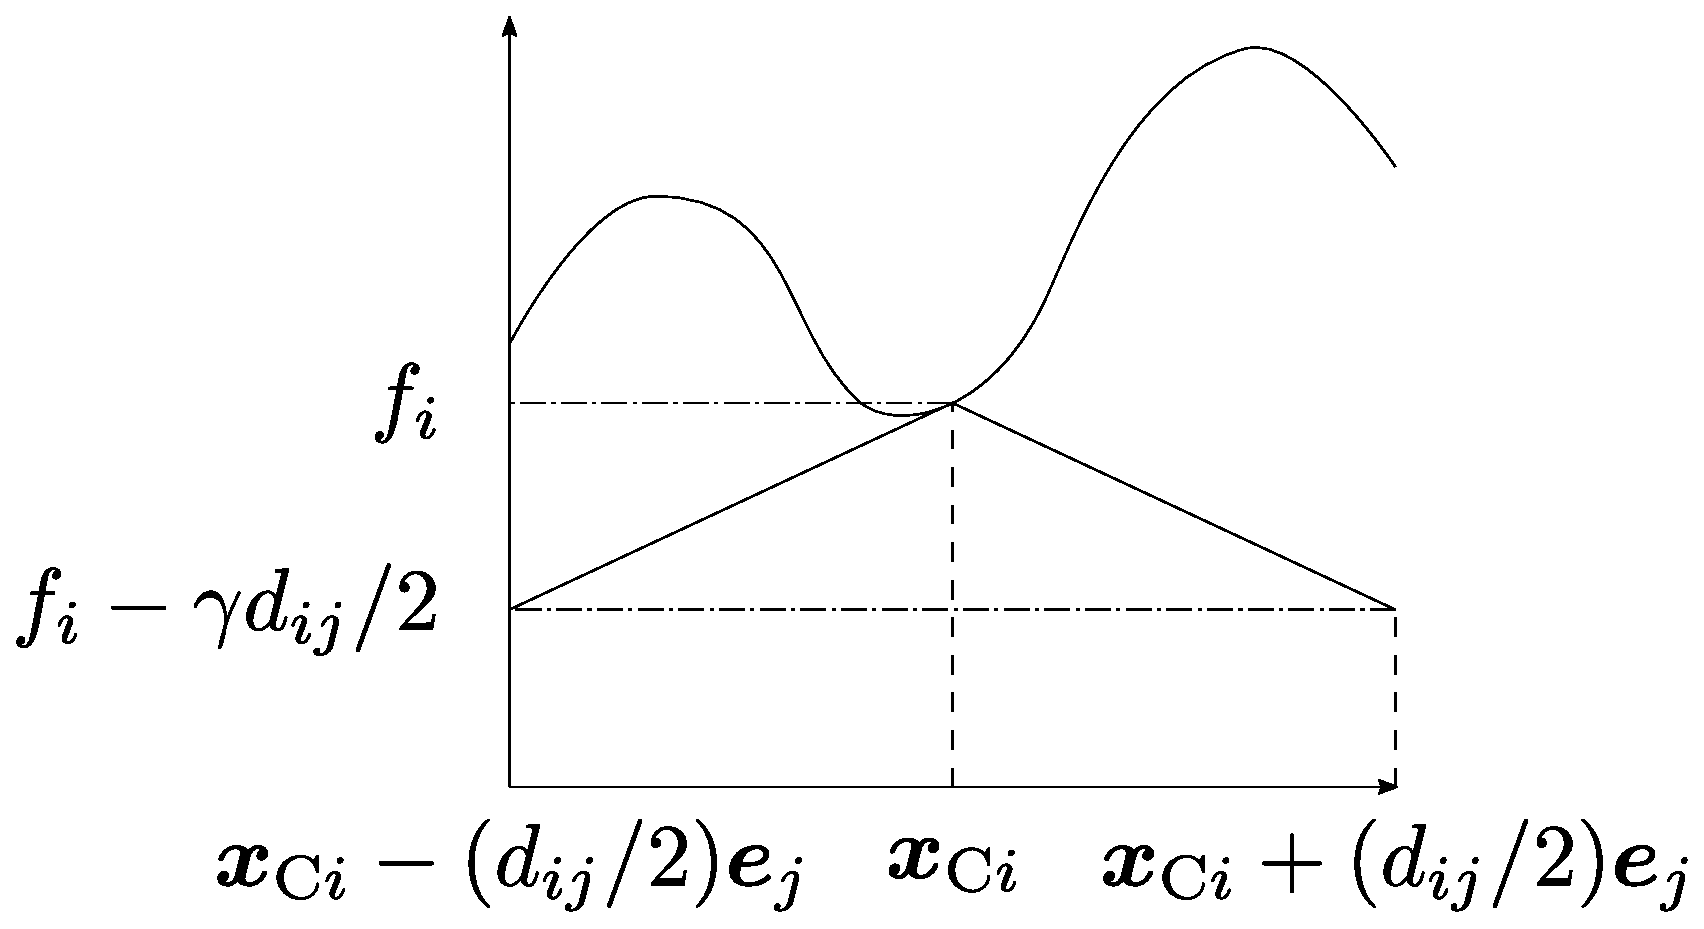
\includegraphics[width=.7\textwidth]{fig/DIRECT_lipschitz_lowerbound.eps}
\end{center}
\end{figure}

全ての次元成分$j=1,\cdots,n$を合わせて考えれば,
\begin{align*}
f(\bm{x})\geq D_{i}\overset{\mathrm{def}}{=}f_{i}-\gamma d_{i}/2
\end{align*}
(ただし$d_{i}\overset{\mathrm{def}}{=}\max_{j}\{d_{ij}\}$)です.

ここで,$x$軸に$d_{i}/2$,$y$軸に$f_{i}=f(\bm{x}_{\mathrm{C}i})$をプロットした図を考えましょう.

\begin{figure}[h]
\begin{center}
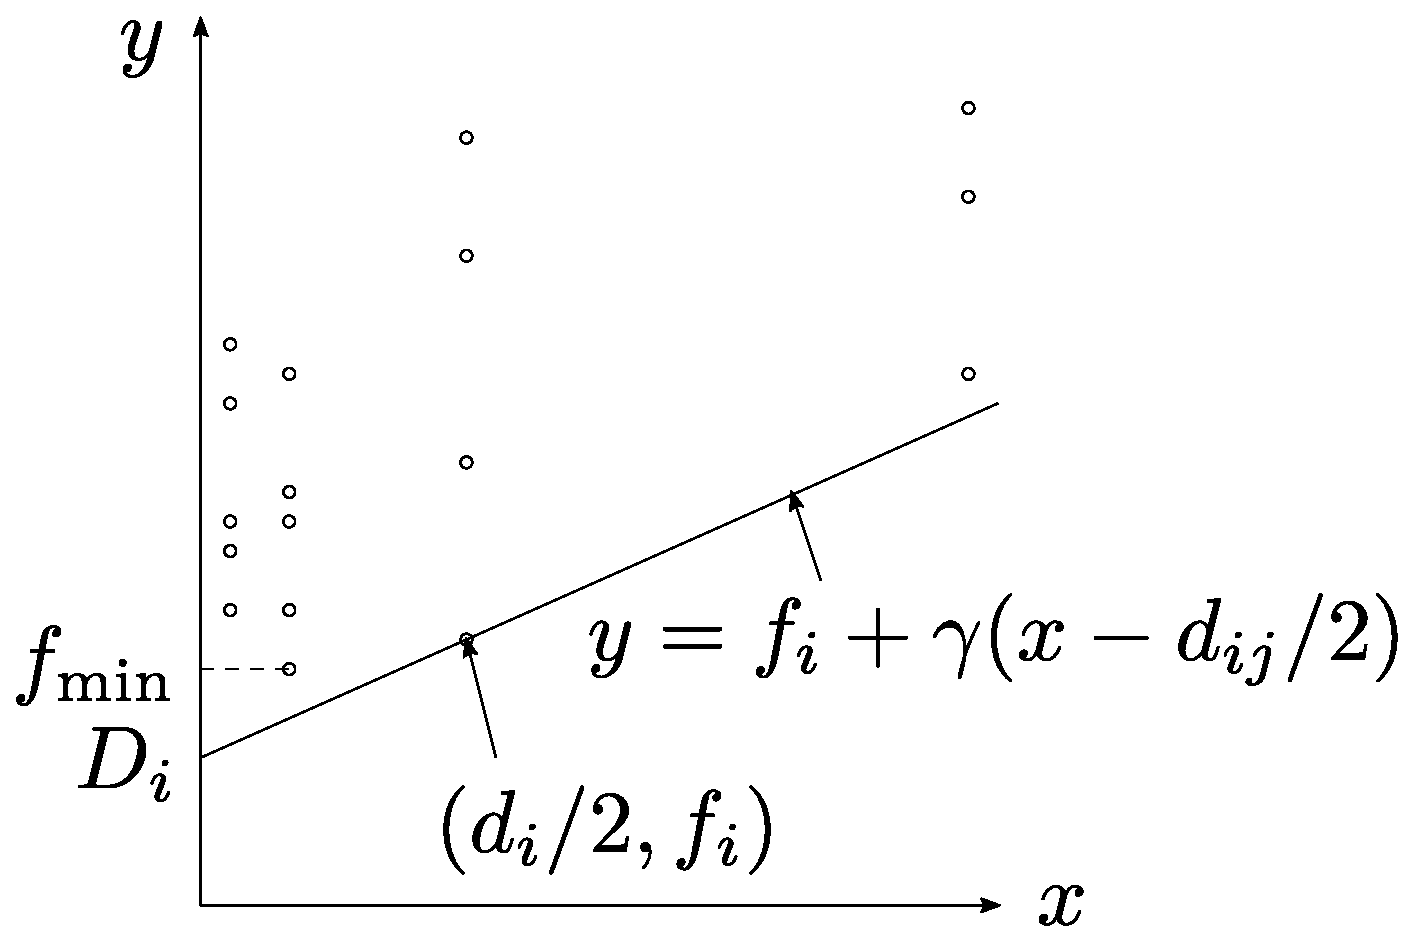
\includegraphics[height=.25\textheight]{fig/DIRECT_lowerbound_estimate.eps}
\end{center}
\end{figure}

点$(d_{i}/2,f_{i})$を通る傾き$\gamma$の直線を引くと,
その$y$軸切片が$D_{i}$となります.
より小さい$D_{i}$を持つ領域ほど,
潜在的に最小点を含む可能性が高いと言えます.
前節で述べた分割方法により,
同一の$d_{i}$すなわち同一のレベルを持つ超長方形領域が複数生成されます.
それらのうち$D_{i}$を最小にするものは,
明らかに,それらの中で$f_{i}$が最小の領域です.

一般的に$\gamma$は未知ですので,
上図のような直線を事前に引くことはできません.
そこで,
「他の全ての領域よりも$D_{i}$を小さくできる可能性のある領域」を{\bf 潜在的最適領域}と呼ぶことにします.
すなわち他の任意の$k$番目領域($k\neq i$)に対して
\begin{align*}
f_{i}-K d_{i}/2 \leq f_{k}-K d_{k}/2
\end{align*}
を満たす正の実数$K$が存在するならば,
$i$番目領域は潜在的最適領域です.
これらは下図における点群の凸包の右下端稜線上頂点に対応する領域(黒丸)に一致します.

\begin{figure}[h]
\begin{center}
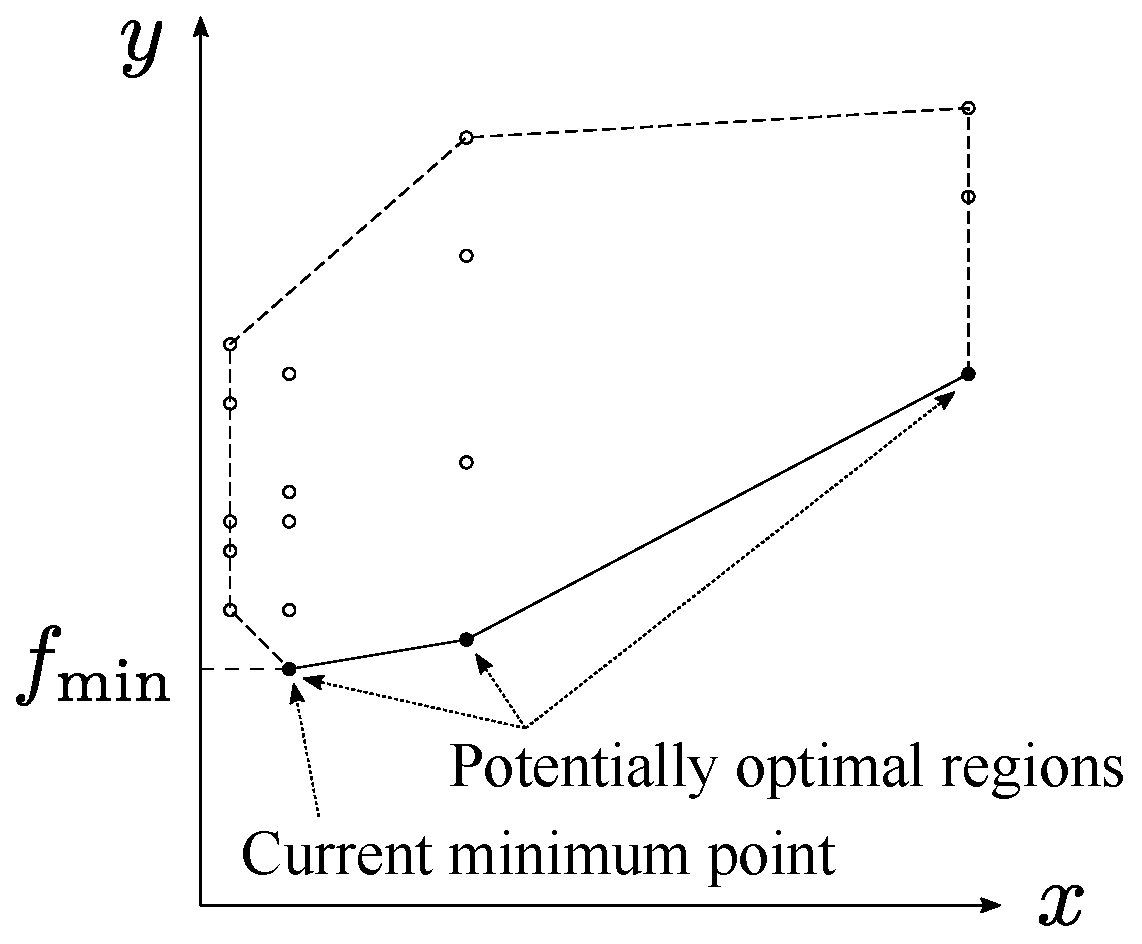
\includegraphics[height=.25\textheight]{fig/DIRECT_POR.eps}
\end{center}
\end{figure}

レベル$l$である領域の数を$N_{l}$とおきましょう.
前節のアルゴリズムによって$\mathcal{R}$が
レベル$l$の超長方形領域群$\mathcal{R}_{l}=\{\bm{\xi}^{(l)}_{1},\cdots,\bm{\xi}^{(l)}_{N_{l}}\}$ごとに分けられ,
$f^{(l)}_{k}$をキーとして昇順にソートされているならば,
潜在的最適領域の候補は$\bm{\xi}^{(0)}_{1},\cdots,\bm{\xi}^{(l_{\mathrm{min}})}_{1}$に絞られます
(ただし$l_{\mathrm{min}}$は$f_{\mathrm{min}}$を与える$l$の値).

なお,出典では
\begin{align*}
f_{i}-K d_{i}/2 \leq f_{\mathrm{min}}-\varepsilon\left|f_{\mathrm{min}}\right|
\end{align*}
を満たす$K$が存在することも潜在的最適領域の条件とされています.
ただし,$f_{\mathrm{min}}=\min_{i}\{f_{i}\}$,$\varepsilon$は設計パラメータです
(経験的に$10^{-4}$程度が良いとされています).
これは最小点探索にあまり貢献しない領域の細分割を避ける目的で設けられているものですが,
精度を下げる原因になるため本稿では採用しません.

潜在的最適領域群$\mathcal{R}_{\mathrm{POR}}$を抽出するアルゴリズムを
Algorithm \ref{alg:direct_ident_por}にまとめます.
Algorithm \ref{alg:direct_find_min}は$\mathcal{R}$から最小値$f_{\mathrm{min}}$およびそれを与える$l_{\mathrm{min}}$を求める処理,
Algorithm \ref{alg:direct_pick_por}は
$\mathcal{R}$から潜在的最適領域$\bm{\xi}$を抽出し$\mathcal{R}_{\mathrm{POR}}$に移す処理です.
$L$は$l$の最大値,
すなわち超長方形の辺長さの最小値を決めるレベルです.
逆に辺長さの最小値を$\varepsilon$程度に設定するならば,
\begin{align*}
3^{-L-1}\leq \varepsilon\leq 3^{-L}
\quad\Leftrightarrow\quad
L\leq -\log_{3}\varepsilon\leq L+1
\quad\Rightarrow\quad
L=\left[-\log_{3}\varepsilon\right]
\end{align*}
とすれば良いです
(ただし,$\lfloor x \rfloor$は$x$を超えない最大の整数を意味します).


\begin{algorithm}[tbh]
\caption{\textsc{DIRECT\_IdentPOR}$(\mathcal{R})\rightarrow(\mathcal{R}_{\mathrm{POR}},f_{\mathrm{min}})$}
\label{alg:direct_ident_por}
\begin{algorithmic}[1]
\State $\mathcal{R}_{\mathrm{POR}}\leftarrow\emptyset$
\State $(l_{\mathrm{min}},f_{\mathrm{min}})\leftarrow$\textsc{DIRECT\_FindMin}$(\mathcal{R})$
\If{$l_{\mathrm{min}}=L$}
  \State \Return{$(\mathcal{R}_{\mathrm{POR}},f_{\mathrm{min}})$}
\EndIf
\State $l\leftarrow 0$
\While{$\mathcal{R}_{l}=\emptyset$}
  \State $l\leftarrow l+1$
\EndWhile
\While{true}
  \State $(\bm{\xi},f)\leftarrow$\textsc{DIRECT\_PickPOR}$(\mathcal{R},\mathcal{R}_{\mathrm{POR}};l)$
  \State TRY:
  \If{$l=l_{\mathrm{min}}$}
    \State break
  \EndIf
  \State $g_{\mathrm{max}}\leftarrow 0$
  \State $l^{\prime}\leftarrow l+1$
  \For{$m\leftarrow l+1,\cdots,l_{\mathrm{min}}$}
    \If{$\mathcal{R}_{m}\neq\emptyset$}
      \State $g\leftarrow\frac{3^{l}\cdot(f-f^{(m)}_{1})}{1-3^{l-m}}$
      \If{$g\geq g_{\mathrm{max}}$}
        \State $g_{\mathrm{max}}\leftarrow g$
        \State $l^{\prime}\leftarrow m$
      \EndIf
    \EndIf
  \EndFor
  \State $l\leftarrow l^{\prime}$
\EndWhile
\State \Return{$(\mathcal{R}_{\mathrm{POR}},f_{\mathrm{min}})$}
\end{algorithmic}
\end{algorithm}

\begin{algorithm}[tbh]
\caption{\textsc{DIRECT\_FindMin}$(\mathcal{R})\rightarrow(l_{\mathrm{min}},f_{\mathrm{min}})$}
\label{alg:direct_find_min}
\begin{algorithmic}[1]
\State $l_{\mathrm{min}}\leftarrow 0$
\State $f_{\mathrm{min}}\leftarrow f^{(0)}_{1}$
\For{$l=1,\cdots,L$}
  \If{$\mathcal{R}_{l}\neq\emptyset$ and $f^{(l)}_{1}<f_{\mathrm{min}}$}
    $l_{\mathrm{min}}\leftarrow l$
    $f_{\mathrm{min}}\leftarrow f^{(l)}_{1}$
  \EndIf
\EndFor
\State \Return{$(l_{\mathrm{min}},f_{\mathrm{min}})$}
\end{algorithmic}
\end{algorithm}

\begin{algorithm}[tbh]
\caption{\textsc{DIRECT\_PickPOR}$(\mathcal{R},\mathcal{R}_{\mathrm{POR}};l)\rightarrow(\bm{\xi},f)$}
\label{alg:direct_pick_por}
\begin{algorithmic}[1]
\State $\bm{\xi}\leftarrow\bm{\xi}^{(l)}_{1}$
\State $f\leftarrow f^{(l)}_{1}$
\State $\mathcal{R}\leftarrow\mathcal{R}-\{\bm{\xi}\}$
\State $\mathcal{R}_{\mathrm{POR}}\leftarrow\mathcal{R}_{\mathrm{POR}}\cup\{\bm{\xi}\}$
\State \Return{$(\bm{\xi},f)$}
\end{algorithmic}
\end{algorithm}



\section{アルゴリズム完成}

これで完成したDIRECT法のアルゴリズムを\textbf{Algorithm \ref{alg:direct}}に示します.

\begin{algorithm}[tbh]
\caption{\textsc{DIRECT}$(f)\rightarrow(\bm{x}^{*},f_{\mathrm{min}})$}
\label{alg:direct}
\begin{algorithmic}[1]
\State \textsc{DIRECT\_Init}$(\mathcal{R};f)$
\State $k\leftarrow 0$; $m\leftarrow 0$
\While{$k<N_{\mathrm{Imax}}$ and $m<N_{\mathrm{Fmax}}$}
  \State $(\mathcal{R}_{\mathrm{POR}},f_{\mathrm{min}})\leftarrow$\textsc{DIRECT\_IdentPOR}$(\mathcal{R})$
  \If{$\mathcal{R}_{\mathrm{PRO}}=\emptyset$}
    \State $\bm{x}^{*}\leftarrow\bm{x}^{(l_{\mathrm{min}})}_{\mathrm{C}1}$
    \State \Return{$(\bm{x}^{*},f_{\mathrm{min}})$}
  \EndIf
  \While{$\mathcal{R}_{\mathrm{POR}}\neq\emptyset$}
    \State $(l_{i},\bm{\xi}_{i})\in\mathcal{R}_{\mathrm{POR}}$
    \State \textsc{DIRECT\_Divide}$(\mathcal{R};l_{i},\bm{\xi}_{i},f)$
  \EndWhile
\EndWhile
\end{algorithmic}
\end{algorithm}

\begin{algorithm}[tbh]
\caption{\textsc{DIRECT\_Init}$(\mathcal{R};f)$}
\label{alg:direct_init}
\begin{algorithmic}[1]
\State $\bm{x}_{\mathrm{C}0}\leftarrow[1/2~~1/2~~\cdots~~1/2]^{\mathrm{T}}$
\For{$j\leftarrow 1,\cdots,n$}
  \State $l_{0j}\leftarrow 0$
\EndFor
\State $f_{0}\leftarrow f(\bm{x}_{\mathrm{C}0})$
\State \textsc{DIRECT\_AddRect}$(\mathcal{R},0,\bm{\xi}_{0})$
\end{algorithmic}
\end{algorithm}


\end{document}
